% Chapter 1

\chapter{Introduzione} % Main chapter title

\label{Chapter1} % For referencing the chapter elsewhere, use \ref{Chapter1} 

\lhead{Capitolo 1. \emph{Introduzione}} % This is for the header on each page - perhaps a shortened title

La prima parte di questa relazione vuole presentare al lettore il contesto di lavoro dell'azienda ospitante il progetto di stage.

%----------------------------------------------------------------------------------------


\section{Azienda}
\begin{figure}[h]\centering  

\includegraphics[scale=0.38]{/home/nicgen/Scrivania/thesis/Figures/logo_sanmarco.png}
\caption[Logo Aziendale]{Logo Aziendale}
\label{pic-a}
\end{figure}

Nata negli anni '80 come software house specializzata negli applicativi per aziende manifatturiere, SanMarco Informatica (http://www.sanmarcoinformatica.it/) è una società italiana che mira principalmente allo sviluppo di software gestionali. Con l'aumento esponenziale della telefonia mobile e dell'internet in mobilità (attraverso smartphone), è stata resa evidente la necessità di ripensare al modo in cui interfacciarsi con il cliente Business. Oltre alle transizioni B2B (Business-to-Business), SanMarco valuta la creazione di particolari software, commissionati da clienti già acquisiti, che possa permettere al pubblico di conoscere meglio il prodotto venduto. 

Nello specifico il progetto aziendale richiedeva la creazione di un software per un cliente del settore oculistico, attraverso il quale un potenziale cliente potesse:

\begin{itemize}
\item Scegliere gli occhiali preferiti da una lista presente sullo schermo dello smarthphone
\item Provare attraverso un feedback visivo, in realtà aumentata, tali occhiali
\item Condividere attraverso i Social Networks una fotografia eventualmente scattata
\end{itemize}

Dato che l'azienda ospitante non possedeva un background in tali ambiti (rilevamento facciale ed integrazione social su piattaforme mobile native), è nata l'esigenza di effettuare uno studio di fattibilità. Nonostante la novità e la natura del progetto, sono state utilizzate tecnologie alternative ma sono state comunque adottate le fasi di sviluppo tipicamente seguite dall'azienda.

\section{Progetto}

\section{Processi Interni}

Le fasi di sviluppo di progetto seguite dall'azienda sono, per ordine:
\begin{itemize}

\item Coordinamento e Riunioni. In questa fase vengono pianificate tutte le attività necessarie allo
svolgimento del progetto.
\item Analisi dei requisiti. L'output dell'attività di analisi è un documento in cui vengono racchiusi
tutti i requisiti funzionali, qualitativi, prestazionali e dichiarativi dei quali il prodotto finale
dovrà garantirne il soddisfacimento. Il documento serve da input per la fase di progettazione
\item Progettazione. Nella fase di progettazione si definiscono le specifiche tecniche delle funzionalità
da realizzare. Il risultato di questa fase è il documento di Specifiche Tecniche di Progettazione
\item Stadio esecutivo del progetto con il quale si realizzano i moduli software previsti
\item Test funzionali e di sistema. I test funzionali hanno lo scopo di verificare che i moduli realizzati
durante la fase di codifica rispettino quanto fissato dai requisiti iniziali. Il test di sistema valida
il prodotto nella sua interezza
\item Collaudo con il cliente. Si tratta di un test di sistema effettuato su un ambiente del cliente
e con dati di prova forniti dallo stesso. L'output di questa attività è un verbale che racconta
l'esito del collaudo
\item Documentazione di prodotto. Questa fase prevede la stesura dei Manuali di Prodotto relativi
al software realizzato
L'output di ogni fase viene verificato e, se conforme agli standard qualitativi dell'azienda, approvato.
Altrimenti dovranno essere indicate delle misure correttive per i problemi individuati
\end{itemize}
\begin{figure}[h]\centering  
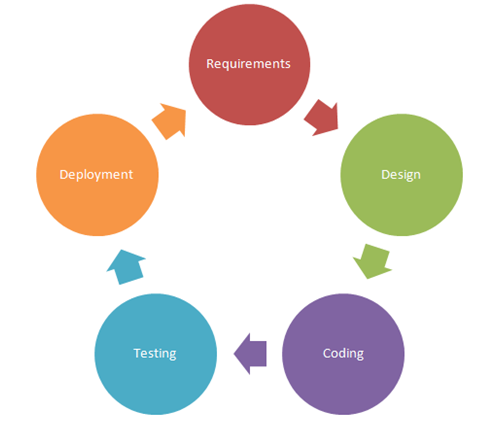
\includegraphics[scale=0.62]{/home/nicgen/Scrivania/thesis/Figures/lifecycle.png}
\caption[Modello di ciclo di vita aziendale]{Modello di ciclo di vita aziendale}
\label{pic-a}
\end{figure}


%----------------------------------------------------------------------------------------

